%%=================== Compiler Directives =================%%
%%                                                         %%
% !TeX program = pdflatex
% !TeX encoding = utf8
% !BIB TS-program =bibtex8
%%                                                         %%
%%=========================================================%%


%%===================== Class Options =====================%%
%%                                                         %%
%%                                                         %%
\documentclass{ConfFTI}



%%===================== Package Placing ===================%%

% \usepackage[most]{tcolorbox}
\usepackage{makecell}
\usepackage{booktabs}
\usepackage{tabularx}
\usepackage{mathtools}
\usepackage{dsfont}
\usepackage{mathrsfs}
\usepackage{wrapfig}
\usepackage{xurl}

%%================== Команди користувача ==================%%
%%            Тут можна визначити власні команди           %%
\DeclareMathOperator{\R}{\mathbb{R}}
\DeclareMathOperator{\N}{\mathbb{N}}
\DeclareMathOperator{\E}{\mathbb{E}}

\newcolumntype{M}[1]{>{\centering\arraybackslash}m{#1}}
%%=========================================================%%




%%======================= Назва тез =======================%%
%%                                                         %%
%%                                                         %%
\title{Застосування генеративно-змагальних мереж для покращення
якості сегментації супутникових знімків}
%%                                                         %%
%%                                                         %%
%%=========================================================%%



%%======================== AUTHORS ========================%%
\author[\email]{О.~В.~Шкаліков}{1} % Команда \email --- вставляє значення наведене в реєстраційній формі

\author{A.~О.~Охріменко}{1}

\author{Л.~Л.~Шуміло}{2}

\author{Н.~М.~Куссуль}{1, 3}

%%========= Назви установ, в яких працюють автори ==========%%

\affiliation{\ntuuipt}{1}
%% Тут введіть установув якій працює, або навчається перший автор.
%% Введіть \ntuu якщо автор навчається, або працює в НТУУ "КПІ"
%% Введіть \ntuuipt якщо автор навчається, або працює в Фізико-технічному інституті
\affiliation{University of Maryland}{2}
\affiliation{Інститут космічних досліджень НАНУ ДКАУ}{3}
%% Тут введіть установу в якій працює, або навчається другий автор



%%================== Реєстраційна форма ===================%%
%%                                                         %%
%%                                                         %%
\FullName{Шкаліков Олег Володимирович}                            %% Повне ім'я доповідача (перший автор)
\Birthday{28.02.2001}                                      %% Дата народження доповідача
\Position{студент}                                        %% Посада доповідача
\phone{+380971864354}                                      %% Телефонний номер доповідача
\authoremail{oleshk-ipt22@lll.kpi.ua}                           %% Email доповідача
\confsection{Математичне модулювання та аналіз даних}                   %% Секція конференції, на яку подається доповідь
\copynum{0}                                                %% Кількість копій збірника матеріалів, необхідних автору 0/1/2 тощо
\NeedLiving{ні}                                           %% Потреба в житлі (Ні/Хостел/Готель/інше)
\NeedInvitation{ні}                                       %% Чи потрібне запрошення на конференцію?
%%                                                         %%
%%                                                         %%
%%=========================================================%%



%%============ Тут вводьте номери PACS або УДК ============%%
%%                                                         %%
%\pacs{ }
\udc{51-74}
%%                                                         %%
%%=========================================================%%



%%============= Тут заповніть ключові слова ===============%%
\keywords{семантична сегментація, UNET,
генеративно-змагальні мережі, Pix2Pix,
незбалансованість класів}

\abstract{%
	Анотація (лат. \textit{annotatio} -- зауваження, помітка) -- короткий виклад змісту статті.
	Дозволяє робити висновки про доцільність їх докладнішого вивчення.%
}



%%====================================================================================%%
\begin{document}


%%=========Замість слова ukrainian (russian, english) введіть мову ваших тез =========%%
%%                                                                                    %%
\PaperLanguage{ukrainian} %
%%                                                                                    %%
%%====================================================================================%%


%%====================================================================================%%
\section*{Вступ}
%%====================================================================================%%
У сучасному світі задачі сегментації супутникових знімків мають
широке прикладне значення, і використовуються для
побудов мап сільськогосподарських культур \cite{kussul2017deep}, детектування незаконної
вирубки лісів \cite{sat_logging}, звалищ, пожеж, тощо. Проте сучасні методи
розв'язку цієї задачі здебільшого є алгоритмами навчання з учителем
та потребують розмічених навчальних вибірок. Створення даного матеріалу,
а саме ground truth масок для навчання потребує значних людських ресурсів, натомість
велика кількість людино-годин може не призвести до значного покращення
результатів сегментації. До того ж, навіть при використанні
такого підходу, точність класифікації міноритарних класів
є низькою, це пов'язано з тим, що загальна площа, яку вони займають
на супутникових знімках з вибірки мала, тому функціонал похибки
роботи моделі не достатньо штрафує за неправильну класифікацію.
Тож пошук методів подолання цих проблем за допомогою генеративно-змагальних
мереж і є метою даного дослідження.

%%====================================================================================%%
\section{Задача семантичної сегментації супутникових знімків}
%%====================================================================================%%

Як і інші задачі навчання з учителем, задача семантичної сегментації
передбачає існування навчальної вибірки, тобто набору $X$,
який складається з зображень
$I \in \left( R^C \right)^{H \times W} = \mathcal{I}$ та міток класів
$k \in K$ для кожного пікселя кожного зображення, де $R \subset \R$ --
множина можливих значень кожного каналу пікселя,
$H, W, C$ -- висота, ширина та кількість каналів зображення,
$K = \overline{1, M}$ -- множина класів ($M \in \N$ -- кількість класів).
Зазвичай множина $R = \overline{0, \dots, 255}$, або $R = [0, 1]$.

Нехай ми маємо навчальну вибірку $X=(I_i, Y_i)_{i=1}^{N}$,
де $I_i \in \mathcal{I}$, $Y_i \in K^{H \times W}$.
Задача семантичної сегментації полягає у тому, щоб
знайти таке відображення
$f: \mathcal{I} \rightarrow K^{H \times W}$, що деякий функціонал помилки
$L(f, X)$ приймає мінімальне значення.

Тобто задача семантичної сегментації є задачею класифікації, але
не цілого зображення, а кожного окремого пікселя.

\section{Проблеми, що виникають при застосуванні нейромережевих підходів}

Попри використання сучасних нейромережевих
архітектур, при розв'язку задач
семантичної сегментації супутникових знімків
виникають істотні проблеми, які не дозволяють
досягти максимальної якості. Ці перепони
є наслідком самої структури задачі, а саме того, що
семантична сегментація є задачею навчання з учителем, тобто вимагає розміченого
набору даних, де кожному супутниковому знімку буде
відповідати відповідна ground-truth маска сегментації.

Тож першою істотною проблемою є те, що створення
навчальних вибірок, а саме: розмітка супутникових знімків,
вимагає значної кількості людських ресурсів. Причому кінцева
якість сегментації безпосередньо залежить від
розміру тренувального набору. Тобто потреба у
покращені значень метрик вимагає, серед усього іншого,
істотного збільшення навчальних прикладів,
а отже й створених людьми ground-truth масок.
Крім того, у випадку створення масок для супутникових знімків,
не завжди людина може правильно класифікувати усі об'єкти ґрунтуючись
тільки на зображенні, що може бути пов'язано з порою року,
розміром об'єкту, роздільною здатністю знімка, схожістю різних класів, тощо.

Друга істотна проблема пов'язана з дуже сильною
незбалансованістю класів, особливо у задачах класифікації
сільськогосподарських культур. Як доказ цього, можна
навести статистику (рис. \ref{fig:pixels_per_class}) ground truth
маски по кількості пікселів по кожному з
типів полів та кількості зображень, отриманих після
поділу композиту на частини по $256 \times 256$ пікселів
на яких представлений даний клас для Київської області.
Вищезгаданий поділ обумовлений тим, що нейромережеві моделі не
можуть ефективно працювати з дуже великими зображеннями,
тож ми вимушені різати їх на частини.

\begin{figure}[ht!]
	\centering
	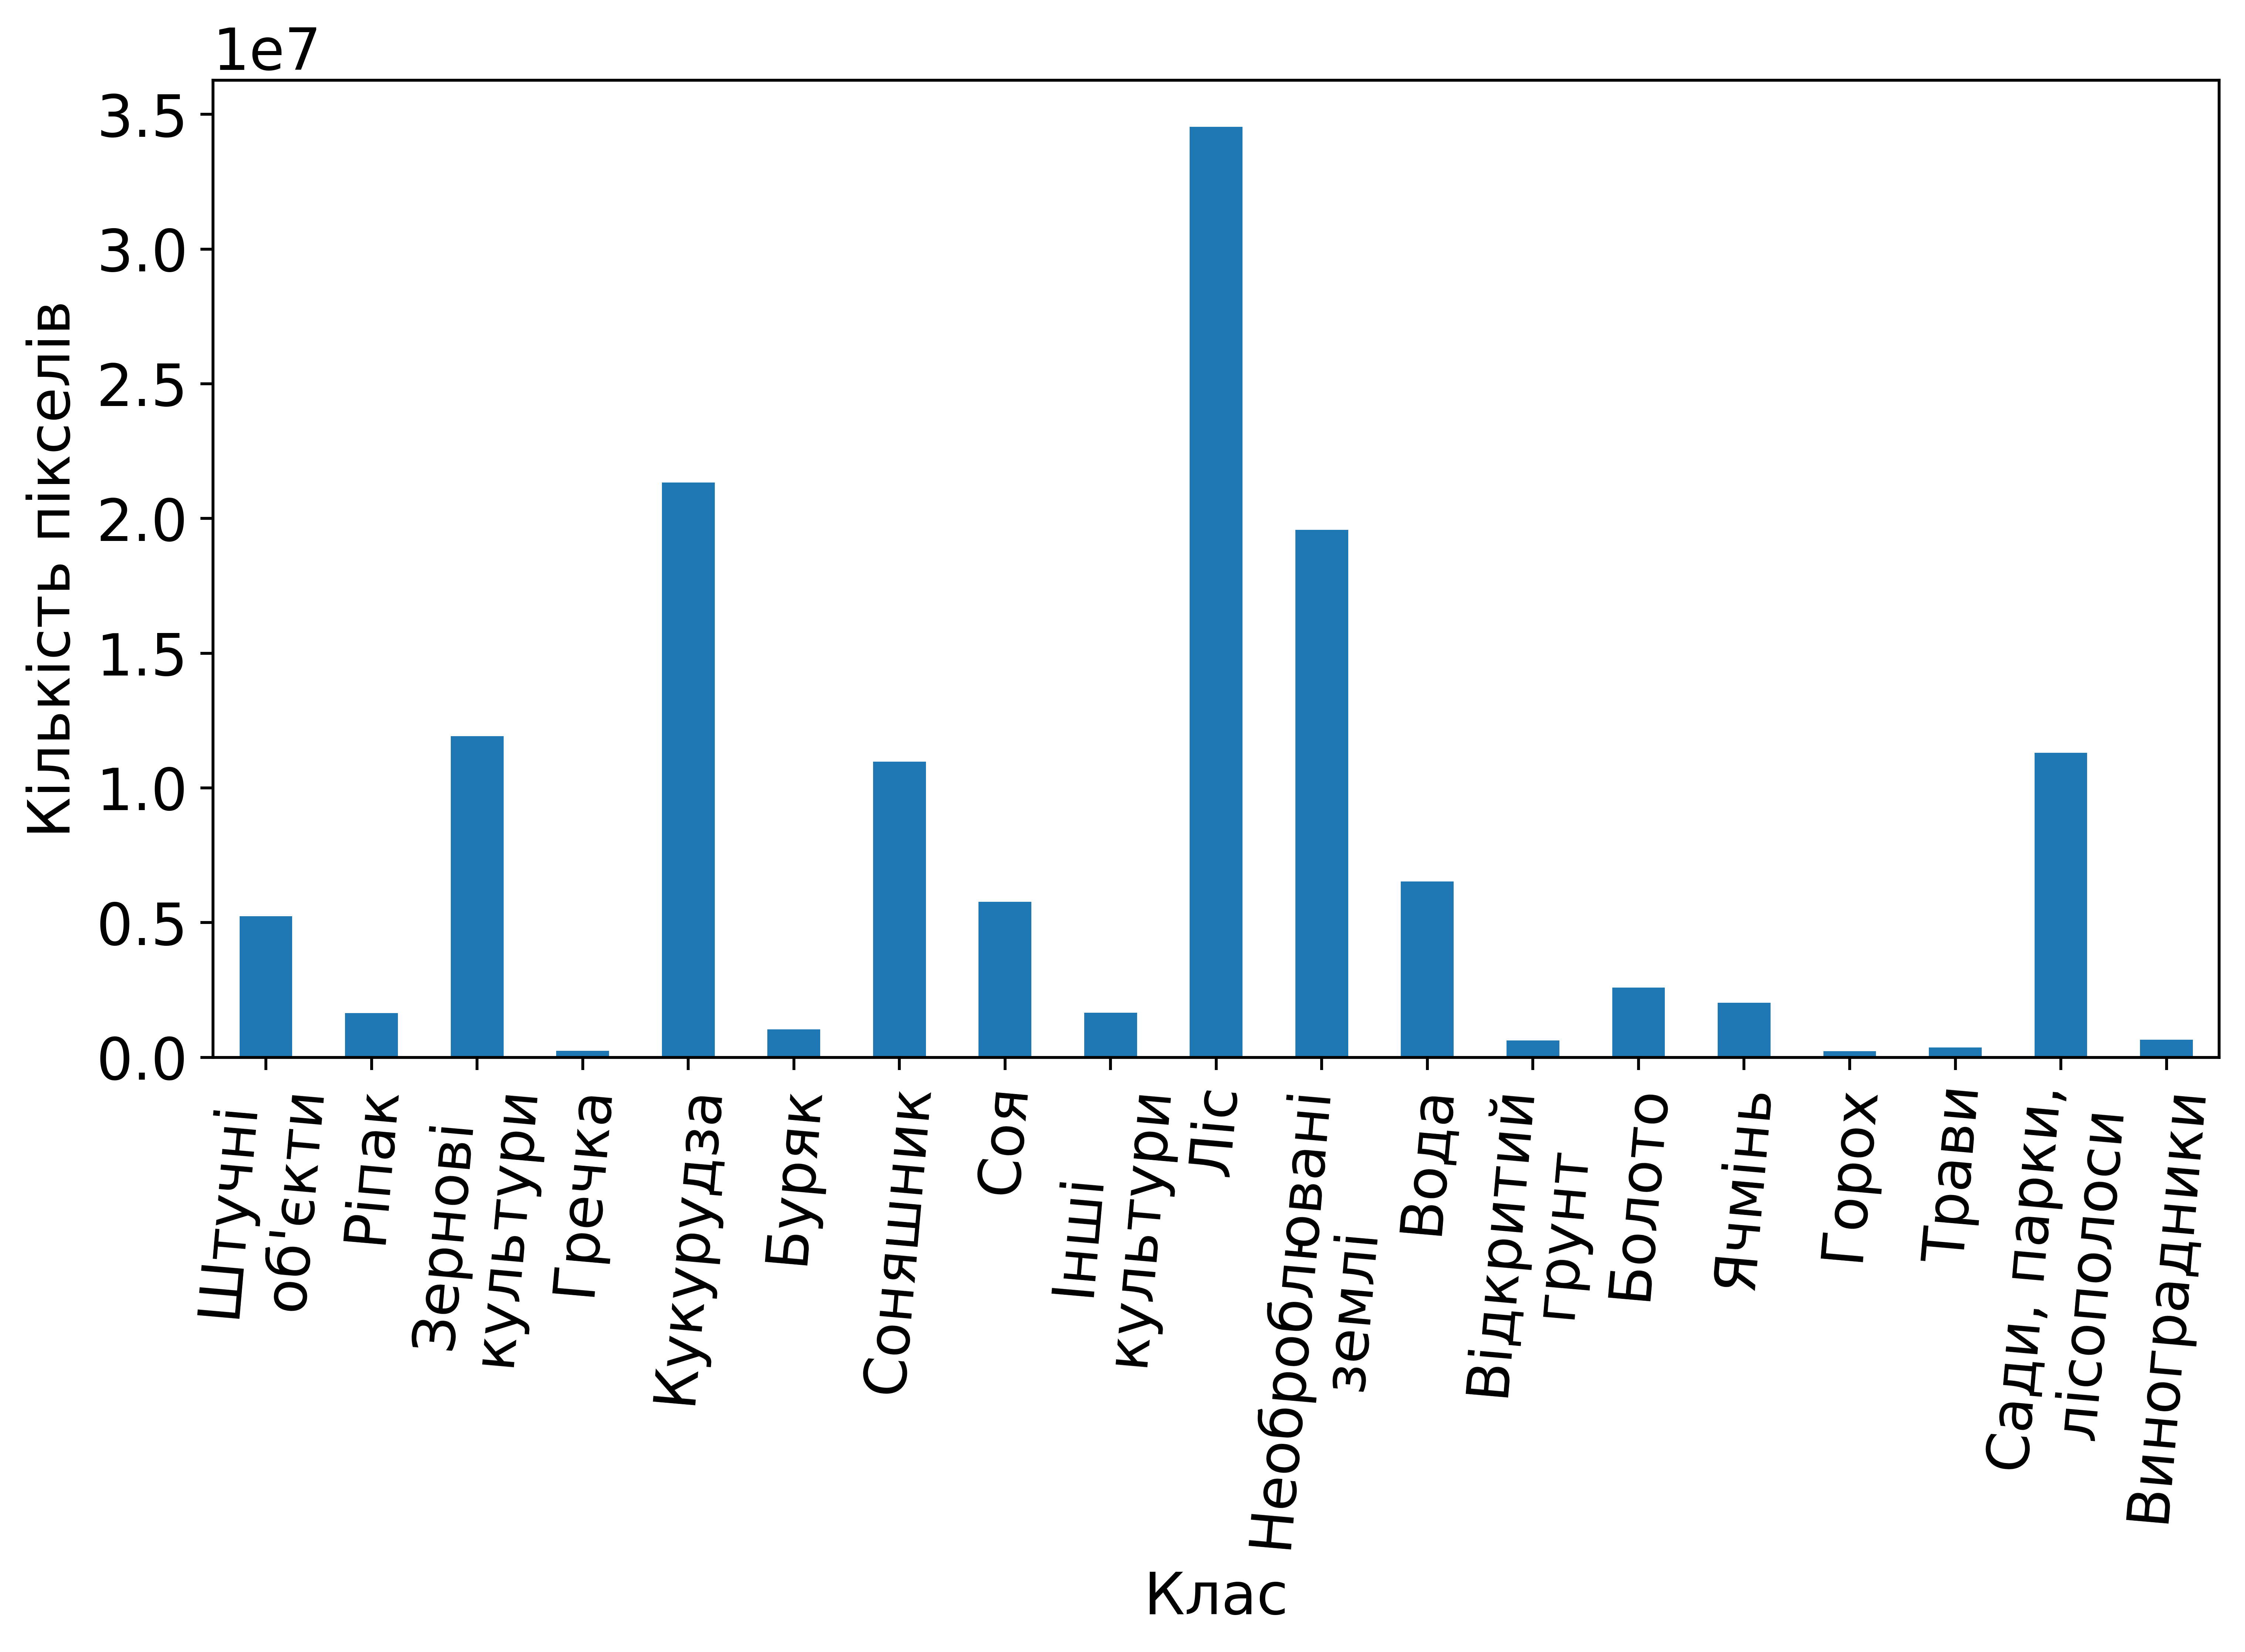
\includegraphics[width=0.49 \textwidth]{assets/dist_real.png}
	\caption{Статистики для різних класів сільськогосподарських культур}
	\label{fig:pixels_per_class}
\end{figure}

І попри застосування
функцій помилок, які можуть враховувати дисбаланс у
класах, досягнути бажаних значень метрик, що описують точність
моделей не вдається.
Особливо незадовільні результати виникають саме для класів,
які мають маленьку кількість прикладів у навчальній вибірці.
А доповнити навчальну вибірку достатньою кількістю
прикладів для певних класів може бути взагалі неможливо,
через особливості сільського господарства у досліджуваному регіоні
або самої сільськогосподарської культури. Останній факт як раз
і є специфічним саме для аналізу супутникових знімків і
виділяє їх серед усіх інших сфер,
де розв'язується задача семантичної сегментації.

\section{Генеративно-змагальні мережі}

Ідея оригінального GAN  \cite{goodfellow2014generative}
полягає у тому, що ми маємо дві сутності:
генератор --- диференційовну функцію $G: Z \times \Theta_G \rightarrow X$, яка
на основі елементу з множини $Z$(шуму, або у деяких випадках,
так званого латентного простору) та параметрів $\theta_g \in \Theta_G$
генерує елемент з множин $X$; та дискримінатор
--- диференційовну функцію $D: X \times \Theta_D \rightarrow \{0, 1\}$, яка
намагається на визначити чи є елемент штучно згенерованим, чи
належить розподілу навчальних даних. Для пошуку функції
генератора та дискримінатора застосовується міні-максний функціонал якості:
$$ \min\limits_{G}\max\limits_{D}
	\E_{x \sim p_{data}} \log D(x) +
	\E_{z \sim p_{z}} \log (1 - D(G(z))) $$

\section{Застосування GAN у задачі Image-to-Image Translation}

У нашому випадку, застосування класичної GAN, запропонованої
у \cite{pix2pix} не є доцільним, бо ті зображення,
що модель повинна продукувати, повинні бути обумовлені
тієї маскою, що подається на вхід системи,
а не тільки випадковим шумом $z$, що обумовлено нашим
намаганням повністю контролювати розподіл класів
у штучно-згенерованих знімках. Тож треба
застосовувати Conditional GAN, одним з широко відомі та поширених
представників яких є Pix2Pix. Схематично його
архітектура виглядає наступним чином (рис. \ref{fig:pix2pix}):

\begin{figure}[ht]
	\centering
	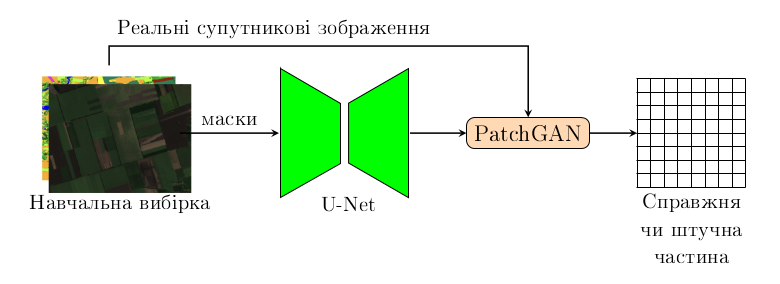
\includegraphics[width= 0.49 \textwidth]{assets/Pix2Pix.png}
	\caption{Архітектура Pix2Pix у застосуванні до супутникових знімків}
	\label{fig:pix2pix}
\end{figure}

У якості функціоналу похибки пропонується використовувати наступний вираз, який являє собою
класичну похибку трансформовану для відповідності Conditional GAN й додаток, який
вимірює схожість згенерованого й реального знімка:
\begin{multline*}
	L(G, D) = \E_{x, y} \log D(x,y) + \\
	\E_{x, z} \log (1 - D(x, G(x, z))) + \\
	\lambda \E_{y, x, z} ||y - G(x, z)||_1
\end{multline*}

Тут, як і у інших Conditional GAN, генератор вже являє собою відображення
$G: X \times Z \rightarrow Y$, а дискримінатор $D: X \times Y \rightarrow \{0, 1\}^{N \times N}$,
де $X$ --- множина масок, $Y$ --- множина супутникових знімків.

Генератором у архітектурі Pix2Pix виступає різновид
мережі UNet \cite{unet}. У якості дискримінатора використовується PatchGAN \cite{pix2pix}, тобто
дискримінатор повертає свій висновок про те є зображення реальним чи штучним не для
усього зображення, а окремо для його частин.

\begin{figure}[ht]
	\centering
	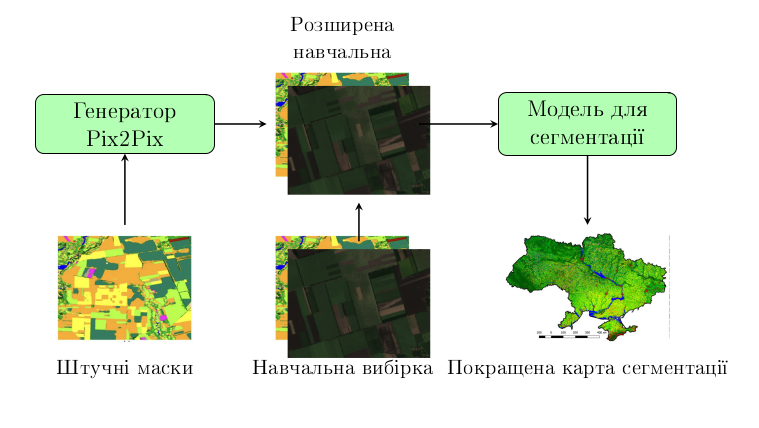
\includegraphics[width=0.49 \textwidth]{assets/pipline.png}
	\caption{Процес аугментації наборів даних супутникових знімків за допомогою Pix2Pix}
	\label{fig:pipline}
\end{figure}

Остаточно, вихідний робочий процес після навчання GAN і відповідно генератора
можна представити діаграмою (рис. \ref{fig:pipline}). Тобто ми згенеруємо на основі масок, які будуть
коригувати незбалансованість класів штучні супутникові знімки,
додамо їх до навчальної вибірки і вже на цьому аугментованому
наборі даних будемо вчити моделі семантичної сегментації.

\section{Дослідження ефективності запропонованого підходу}

Для перевірки того, чи дійсно запропонований підхід
дозволить збільшити якість семантичної сегментації супутникових знімків
було проведено експерименти по класифікації на 19 класів
(здебільшого сільськогосподарських культур) композиту Sentinel-2A \cite{drusch2012sentinel}
для Київської області взятих з 1 липня по 1 серпня 2021 року.

Попередня обробка даних включала в себе поділ композиту на
зображення $256 \times 256$ пікселів, видалення зображень у яких
відсутні дані про деякі пікселі чи мітка класу, а також нормалізація з
параметрами $0.5$ у якості середнього та $0.5$ у якості стандартного відхилення,
для усіх каналів кожного пікселя. Набір даних було поділено навпіл
на навчальну та тестову вибірки.

Після цього було навчено генеративно-змагальну мережу архітектури
Pix2Pix протягом 300 епох. Згенеровано маски за наступним алгоритмом,
у кожній масці вихідного набору даних було змінено $i$-ий за сумарною кількістю
пікселів клас на $(19 - i + 1)$. На основі цих масок, навченою мережею
були згенеровані супутникових знімки. Ці знімки разом з масками були
додані до вихідного набору даних, тобто отримали аугментовану вибірку.

І остаточно було навчено модель UNet \cite{unet} на основі тільки реальних даних
і аугментованої вибірки. Після цього було виміряно точність (producer accuracy).
Результати по кожному з класів наведені у табл. \ref{tab:augm_compare}.

В усіх процесах навчання використовувався оптимізатор Adam \cite{diederik2014adam}
зі швидкістю навчання $2 \cdot 10^{-4}$. При навчанні GAN у якості параметрів
експоненційного середнього $\beta_1, \beta_2$ використовувались
значення $0.5, 0.999$ відповідно.

\begin{table}[ht]
	\centering
	\caption{Порівняльна таблиця точності сегментації по кожному з класів (у процентах)}
	\begin{tabular}{|M{2.5cm}|M{2.5cm}|M{2.5cm}|}
		\hline
		\textbf{Назва класу}              & \textbf{Реальні дані} & \textbf{Аугментована вибірка} \\
		\hline Штучні об'єкти             & 69                    & 71                            \\
		\hline Зернові культури           & 89                    & 79                            \\
		\hline Ріпак                      & 0                     & 53                            \\
		\hline Гречка                     & 0                     & 0                             \\
		\hline Кукурудза                  & 94                    & 87                            \\
		\hline Буряк                      & 0                     & 23                            \\
		\hline Соняшник                   & 89                    & 94                            \\
		\hline Соя                        & 27                    & 66                            \\
		\hline Інші культури              & 0                     & 6                             \\
		\hline Ліс                        & 93                    & 93                            \\
		\hline Необроблювані землі        & 71                    & 76                            \\
		\hline Відкритий ґрунт            & 3                     & 54                            \\
		\hline Вода                       & 97                    & 97                            \\
		\hline Болото                     & 27                    & 34                            \\
		\hline Ячмінь                     & 5                     & 21                            \\
		\hline Горох                      & 0                     & 1                             \\
		\hline Трави                      & 0                     & 0                             \\
		\hline Сади, парки, лісополоси    & 45                    & 50                            \\
		\hline Виноградники               & 0                     & 0                             \\
		\hline \textbf{Загальна точність} & \textbf{75}           & \textbf{79}                   \\
		\hline
	\end{tabular}
	\label{tab:augm_compare}
\end{table}

Як можна побачити точність для мажоритарних класів, таких як
зернові культури або кукурудза трохи зменшилась,
проте у випадку з міноритарними класами ситуація повністю протилежна:
ми змогли досягти значного підвищення якості класифікації саме цих класів.
Тож ми можемо стверджувати, що для міноритарних класів, даний
підхід є ефективним та дозволяє значно покращити якість
семантичної сегментації.


\section*{Висновки}
%%====================================================================================%%

У результаті проведеної роботи була досліджена проблема
семантичної сегментації супутникових знімків, яка має важливу
роль у прикладних застосуваннях. Проте були виявлені та описані
проблеми, які виникають під час розв'язку цієї задачі сучасними
нейромережевими методами, а саме: складність створення великих
вибірок та сильна незбалансованість класів. Причому, на відміну від
інших сфер, отримати навчальні приклади, які могли б змінити розподіл
класів у багатьох випадках для супутникових даних не є можливим.

Для подолання цих проблем було розглянуто можливість аугментації
навчальної вибірки штучно згенерованими навчальними прикладами.
Для цього була дослідженні моделі, які дозволяють вирішити цю задачу,
а саме генеративно-змагальні мережі. При цьому, для вирішення проблеми
незбалансованості класів стандартні GAN не кращий вибір, бо
ми не можемо контролювати розподіл класів на згенерованих зображеннях.
Тому були опрацьовані моделі image-to-image translation, зокрема Pix2Pix,
які дозволяють генерувати супутникові знімки на основі масок.
У свою чергу модифікація вже існуючих масок, тобто зміна одних
класів на інші дозволяє скоригувати незбалансованість класів.

Таким чином було розроблено процес аугментації наборів даних супутникових
знімків, ефективність якого була перевірений експериментальним чином (табл. \ref{tab:augm_compare}).
У результаті ми отримали підтвердження того, що запропонований
підхід дозволяє значно підвищити якість семантичної сегментації
міноритарних класів, при цьому якість класифікації мажоритарних класів, хоч
у деяких випадках і стала нижчою, проте незначно.

Очевидні і подальші напрямки досліджень у даній сфері. По-перше, це
дослідження методів генерації, які б дозволили б врахувати той факт,
що супутникові знімки однієї території у різні пори року значно відрізняються.
По-друге, створення більш досконалих методів генерації масок.
І врешті решт, покращення існуючих генеративно-змагальних мереж
для генерації ще більш реалістичних штучних супутникових знімків.

%%====================================================================================%%
%%                          Оформлення бібліографічних посилань                       %%
%%====================================================================================%%

\bibliographystyle{ugost2008}
\bibliography{Shkalikov}

\raggedend
\end{document}